\documentclass[12pt,a4paper]{article}
\usepackage[utf8]{inputenc}
\usepackage{geometry}
\geometry{top=2.5cm, bottom=2.5cm, left=2.5cm, right=2.5cm}
\usepackage{graphicx}
\usepackage{tikz}
\usetikzlibrary{shapes.geometric, arrows, positioning, fit, backgrounds, arrows.meta}
\usepackage{hyperref}
\usepackage{xcolor}
\usepackage{titlesec}
\usepackage{parskip}
\usepackage{booktabs}
\usepackage{listings}

% Custom Colors
\definecolor{primary}{RGB}{0, 87, 155}
\definecolor{secondary}{RGB}{74, 20, 140}
\definecolor{accent}{RGB}{230, 81, 0}
\definecolor{success}{RGB}{27, 94, 32}

% Title Formatting
\titleformat{\section}{\Large\bfseries\color{primary}}{}{0em}{}[\titlerule]
\titleformat{\subsection}{\large\bfseries\color{secondary}}{}{0em}{}
\titleformat{\subsubsection}{\normalsize\bfseries}{}{0em}{}

% Link Setup
\hypersetup{
    colorlinks=true,
    linkcolor=primary,
    filecolor=magenta,      
    urlcolor=accent,
    pdftitle={IntelliLead Agentic Pipeline Documentation},
}

\begin{document}

\begin{titlepage}
    \centering
    \vspace*{2cm}
    
    {\Huge\bfseries\color{primary} IntelliLead: Advanced Agentic Pipeline \par}
    \vspace{1cm}
    {\Large\itshape Comprehensive Technical & Operational Architecture Report \par}
    \vspace{2cm}
    
    {\Large Prepared for Executive Management \par}
    \vspace{3cm}
    
    \vfill
    
    {\large \today \par}
\end{titlepage}

\tableofcontents
\newpage

% ---------------------------------------------------------
\section{1. Executive Summary & Business Problem}
% ---------------------------------------------------------

In the competitive landscape of B2B lead generation, acquiring high-quality, verified data for niche sectors (such as Event Management and Wedding Planning) represents a massive operational bottleneck. A traditional, manual approach involves:

\begin{itemize}
    \item \textbf{Fragmented Sourcing}: Employees manually searching isolated platforms like Google Maps, JustDial, WedMeGood, and IndiaMART.
    \item \textbf{Unstructured Data}: Copy-pasting unstructured and inconsistent data fields into spreadsheets.
    \item \textbf{Duplication Epidemic}: Identifying whether a business listed on Google Maps is the exact same entity as one listed on JustDial under a slightly different name.
    \item \textbf{Relevance Contamination}: Failing to distinguish between a full-service "Event Planner" and a "Caterer" who happens to appear in the search results.
    \item \textbf{Data Enrichment}: Performing secondary manual web searches to find missing critical information, such as direct contact numbers or Instagram URLs.
\end{itemize}

This manual methodology is prohibitively slow, highly prone to human error, and completely unscalable. 

\textbf{The Solution:} \textit{IntelliLead} was developed as a fully autonomous, AI-driven Agentic Pipeline. It performs massive-scale data extraction via stealth browser automation, mathematically merges duplicates across platforms, utilizes localized Machine Learning to filter out irrelevant leads, and generates a boardroom-ready, enriched database in minutes.

% ---------------------------------------------------------
\section{2. The Role of Antigravity (Agentic AI Assistant)}
% ---------------------------------------------------------

The development, maintenance, and complex architectural structuring of the IntelliLead platform were significantly accelerated by \textbf{Antigravity}, an advanced Agentic AI coding assistant developed by Google DeepMind. 

Unlike traditional code-completion tools or chatbots, Antigravity operates as an autonomous, virtual Senior Software Engineer integrated directly into the development environment.

\subsection{Key Contributions of Antigravity}
\begin{enumerate}
    \item \textbf{Autonomous Engineering}: Antigravity was responsible for reading the entire workspace context and autonomously writing, debugging, and optimizing complex logic, such as the stealth browser configurations in Playwright.
    \item \textbf{Implementation Planning}: Before executing complex tasks (such as refactoring the deduplication logic or generating this documentation), Antigravity created structured \textit{Implementation Plans} for human review, ensuring architectural alignment before modifying the codebase.
    \item \textbf{Environment Execution}: It directly executed terminal commands to run test suites, manage Python package dependencies, and verify the successful generation of output artifacts.
    \item \textbf{Self-Healing and Refactoring}: During the development lifecycle, Antigravity dynamically responded to runtime errors (e.g., Unicode encoding issues in the terminal) by autonomously rewriting and optimizing the affected modules without requiring manual human intervention.
\end{enumerate}

Antigravity ensures that the IntelliLead system remains state-of-the-art, maintainable, and highly adaptable to future platform security changes or business requirements.

% ---------------------------------------------------------
\section{3. System Architecture Diagram}
% ---------------------------------------------------------

The following diagram illustrates the four-phase architecture of the IntelliLead pipeline, from raw web extraction to the final structured presentation.

\vspace{1cm}
\begin{center}
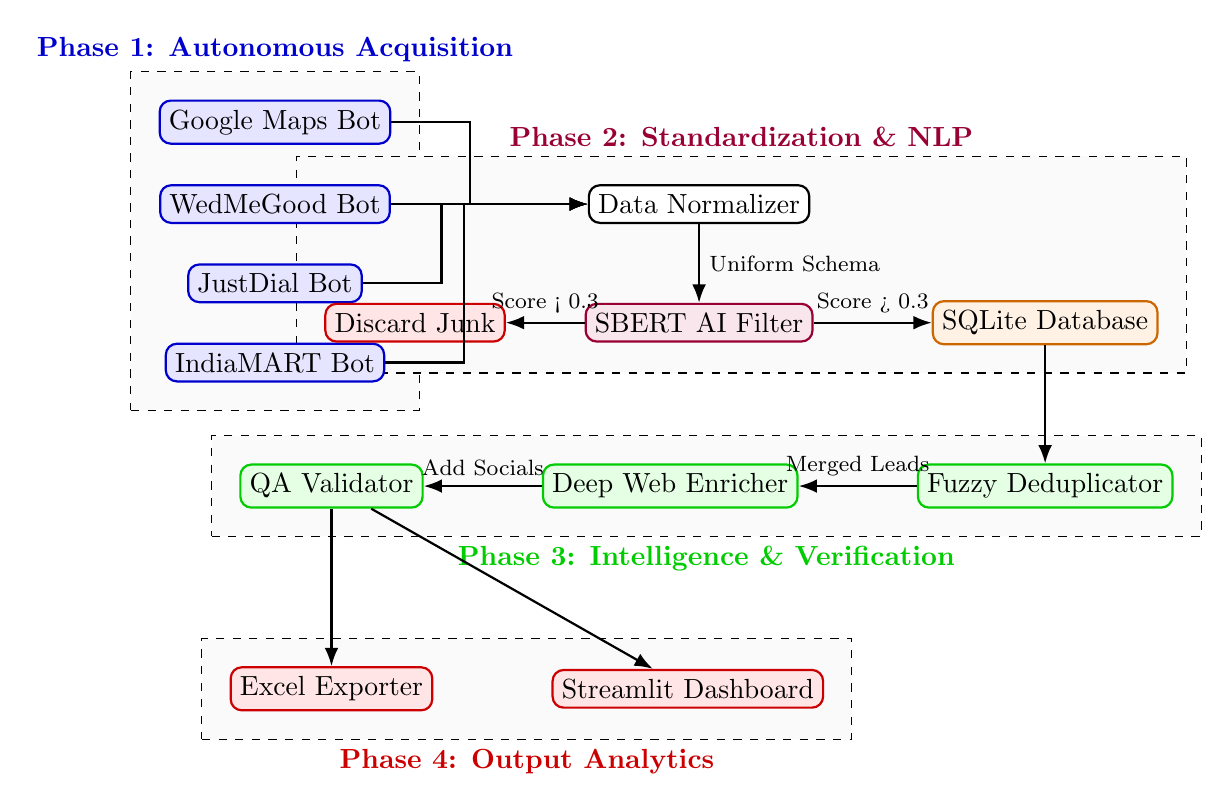
\begin{tikzpicture}[
    node distance=1.5cm and 2cm,
    box/.style={rectangle, draw, rounded corners, align=center, fill=white, thick},
    layer/.style={rectangle, draw, dashed, inner sep=10pt, fill=black!2},
    arrow/.style={-Latex, thick}
]

% Phase 1 Nodes
\node[box, fill=blue!10, draw=blue!80!black] (gmaps) {Google Maps Bot};
\node[box, fill=blue!10, draw=blue!80!black, below=0.5cm of gmaps] (wmg) {WedMeGood Bot};
\node[box, fill=blue!10, draw=blue!80!black, below=0.5cm of wmg] (jd) {JustDial Bot};
\node[box, fill=blue!10, draw=blue!80!black, below=0.5cm of jd] (imart) {IndiaMART Bot};

% Phase 1 Background
\begin{scope}[on background layer]
    \node[layer, fit=(gmaps) (wmg) (jd) (imart), label={[font=\bfseries\color{blue!80!black}]above:Phase 1: Autonomous Acquisition}] (phase1) {};
\end{scope}

% Phase 2 Nodes
\node[box, right=2.5cm of wmg] (norm) {Data Normalizer};
\node[box, fill=purple!10, draw=purple!80!black, below=1cm of norm] (ai) {SBERT AI Filter};
\node[box, fill=red!10, draw=red!80!black, left=1cm of ai] (discard) {Discard Junk};
\node[box, fill=orange!10, draw=orange!80!black, right=1.5cm of ai] (db) {SQLite Database};

% Phase 2 Background
\begin{scope}[on background layer]
    \node[layer, fit=(norm) (ai) (discard) (db), label={[font=\bfseries\color{purple!80!black}]above:Phase 2: Standardization \& NLP}] (phase2) {};
\end{scope}

% Phase 3 Nodes
\node[box, fill=green!10, draw=green!80!black, below=1.5cm of db] (dedupe) {Fuzzy Deduplicator};
\node[box, fill=green!10, draw=green!80!black, left=1.5cm of dedupe] (enrich) {Deep Web Enricher};
\node[box, fill=green!10, draw=green!80!black, left=1.5cm of enrich] (val) {QA Validator};

% Phase 3 Background
\begin{scope}[on background layer]
    \node[layer, fit=(dedupe) (enrich) (val), label={[font=\bfseries\color{green!80!black}]below:Phase 3: Intelligence \& Verification}] (phase3) {};
\end{scope}

% Phase 4 Nodes
\node[box, fill=red!10, draw=red!80!black, below=2cm of val] (excel) {Excel Exporter};
\node[box, fill=red!10, draw=red!80!black, right=1.5cm of excel] (ui) {Streamlit Dashboard};

% Phase 4 Background
\begin{scope}[on background layer]
    \node[layer, fit=(excel) (ui), label={[font=\bfseries\color{red!80!black}]below:Phase 4: Output Analytics}] (phase4) {};
\end{scope}

% Connecting arrows
\draw[arrow] (gmaps.east) -- ++(1,0) |- (norm.west);
\draw[arrow] (wmg.east) -- ++(1,0) |- (norm.west);
\draw[arrow] (jd.east) -- ++(1,0) |- (norm.west);
\draw[arrow] (imart.east) -- ++(1,0) |- (norm.west);

\draw[arrow] (norm) -- node[right, font=\footnotesize] {Uniform Schema} (ai);
\draw[arrow] (ai) -- node[above, font=\footnotesize] {Score < 0.3} (discard);
\draw[arrow] (ai) -- node[above, font=\footnotesize] {Score > 0.3} (db);

\draw[arrow] (db) -- (dedupe);
\draw[arrow] (dedupe) -- node[above, font=\footnotesize] {Merged Leads} (enrich);
\draw[arrow] (enrich) -- node[above, font=\footnotesize] {Add Socials} (val);

\draw[arrow] (val) -- (excel);
\draw[arrow] (val) -- (ui);

\end{tikzpicture}
\end{center}
\vspace{1cm}

% ---------------------------------------------------------
\section{4. Detailed Component \& File Breakdown}
% ---------------------------------------------------------

The IntelliLead codebase is strictly modularized to separate data extraction, structural mapping, intelligence processing, and user interface generation.

\subsection{Root Directory (Orchestration \& Control)}

\subsubsection{\texttt{main.py} (The Orchestrator)}
This is the core execution script. It defines the \texttt{ScraperOrchestrator} class, which acts as the supreme controller. 
\begin{itemize}
    \item \textbf{Usage}: Executed via terminal to trigger massive mining jobs across multiple cities and keywords.
    \item \textbf{Logic}: It loops through the target matrices defined in the configuration, invokes the respective scraper bots sequentially, captures raw data, routes it through the standardizer and AI filter, and saves checkpoints. It features a \texttt{--process-only} flag to skip scraping and only run intelligence algorithms on existing data.
\end{itemize}

\subsubsection{\texttt{app.py} (Streamlit Dashboard)}
\begin{itemize}
    \item \textbf{Usage}: Provides a premium, web-based graphical user interface for management.
    \item \textbf{Logic}: It connects to the SQLite database to display live intelligence discovery feeds and database ingestion metrics. It dynamically loads generated \texttt{.xlsx} files from the \texttt{outputs/} directory, applies color gradients to high-scoring metrics, and provides secure download links for the final reports.
\end{itemize}

\subsubsection{\texttt{config.py} (The Rulebook)}
\begin{itemize}
    \item \textbf{Usage}: Centralizes all system parameters.
    \item \textbf{Logic}: Defines target cities, target keywords, directory paths, rotating user agents for bot-evasion, and crucially, the \texttt{DEDUPE\_THRESHOLDS} (fuzzy logic weights) that dictate exactly how aggressively the system should merge similar businesses.
\end{itemize}

\subsubsection{\texttt{demo\_run.py} (Rapid Demonstration Script)}
\begin{itemize}
    \item \textbf{Usage}: A highly compressed version of \texttt{main.py} used exclusively for live presentations.
    \item \textbf{Logic}: Limits the extraction to a single city (Jaipur) and a strict cap of 5 leads. It runs the entire extraction-to-export pipeline in under 60 seconds to immediately prove system viability to stakeholders.
\end{itemize}

\subsection{The Data Models Layer (\texttt{models/})}

\subsubsection{\texttt{schema.py} (The Data Blueprint)}
\begin{itemize}
    \item \textbf{Usage}: Enforces rigid data structure utilizing Pydantic.
    \item \textbf{Logic}: Defines the \texttt{BusinessSchema} class. Because Google Maps labels a phone number as "Phone:" and JustDial labels it as a custom icon, this schema forces all incoming data into standardized keys (e.g., \texttt{contact\_number}, \texttt{business\_name}, \texttt{instagram\_url}). It also contains the mathematical logic for merging two schema objects together, preserving the highest-quality data fields from both.
\end{itemize}

\subsubsection{\texttt{database.py} (State Management)}
\begin{itemize}
    \item \textbf{Usage}: Manages local persistence using SQLite3.
    \item \textbf{Logic}: Contains the \texttt{DatabaseManager} class. It handles bulk data ingestion and, crucially, implements a Checkpoint tracking system (\texttt{scrape\_checkpoints} table). If a network outage occurs, the system knows exactly which page of which platform in which city it failed on, ensuring zero duplicate work upon restart.
\end{itemize}

\subsubsection{\texttt{duplicate\_matcher.py} (Fuzzy Logic Engine)}
\begin{itemize}
    \item \textbf{Usage}: Identifies duplicate business entities across heterogeneous sources.
    \item \textbf{Logic}: Utilizes the \texttt{rapidfuzz} library. It performs normalized Levenshtein distance calculations on business names (e.g., matching "ABC Events" with "ABC Event Planners" at 85\% confidence) and cross-references phone numbers and addresses to group disjointed records into unified clusters.
\end{itemize}

\subsubsection{\texttt{relevance\_classifier.py} (The AI Filter)}
\begin{itemize}
    \item \textbf{Usage}: Ensures 100\% lead quality by rejecting false positives.
    \item \textbf{Logic}: Initializes a local Sentence-Transformers model (\texttt{all-MiniLM-L6-v2}). It computes the cosine similarity between the scraped business's services and the target intent ("wedding event planning"). If a catering company inadvertently appears in a wedding planner search, the SBERT model calculates a low semantic similarity score and autonomously rejects the lead.
\end{itemize}

\subsection{The Intelligence Pipelines (\texttt{pipelines/})}

\subsubsection{\texttt{normalize.py} (Data Sanitization)}
\begin{itemize}
    \item \textbf{Logic}: Cleans string encodings, strips leading/trailing whitespaces, removes duplicate tags within lists, and ensures the data conforms flawlessly to the \texttt{BusinessSchema} before entering the database.
\end{itemize}

\subsubsection{\texttt{dedupe.py} (Cluster Resolution)}
\begin{itemize}
    \item \textbf{Logic}: Acts as the executor for the \texttt{DuplicateMatcher}. Once duplicate clusters are identified, this pipeline iterates through the clusters and triggers the \texttt{.merge()} method defined in the schema, condensing 3 raw rows into 1 enriched "Super-Lead".
\end{itemize}

\subsubsection{\texttt{enrich.py} (Deep Web Discovery)}
\begin{itemize}
    \item \textbf{Logic}: Acts as an automated private investigator. If a validated lead lacks an Instagram URL or contact number, this pipeline queries DuckDuckGo via HTTP requests, parses the search engine results pages (SERPs), and hunts for official social media footprints or corporate websites to fill the missing voids.
\end{itemize}

\subsubsection{\texttt{validate.py} (Quality Assurance)}
\begin{itemize}
    \item \textbf{Logic}: Applies strict Regular Expression (Regex) patterns to validate the integrity of contact information. It ensures Indian phone numbers contain exactly 10 digits and emails possess valid domain structures. It ultimately assigns a final \texttt{Confidence Score} (Verified, Enriched, Raw, or Low Confidence) based on data density.
\end{itemize}

\subsubsection{\texttt{export\_excel.py} (Report Generation)}
\begin{itemize}
    \item \textbf{Logic}: Transforms the Pydantic objects into Pandas DataFrames. It utilizes \texttt{openpyxl} to apply corporate styling (frozen headers, brand colors, autofilters) and dynamically creates separate spreadsheet tabs for every distinct city, ensuring the final output is instantly ready for sales team distribution.
\end{itemize}

\subsection{The Data Acquisition Layer (\texttt{scrapers/})}

\subsubsection{\texttt{base\_scraper.py} (The Stealth Engine)}
\begin{itemize}
    \item \textbf{Usage}: The foundational class inherited by all specific bots.
    \item \textbf{Logic}: Utilizes Playwright alongside \texttt{playwright-stealth}. It actively mutates the browser fingerprint (overriding \texttt{navigator.webdriver}, injecting randomized User-Agents, spoofing plugins) to prevent detection by advanced bot mitigation systems (like Cloudflare). It also includes algorithmic \texttt{human\_scroll()} functions to trigger lazy-loaded DOM elements naturally.
\end{itemize}

\subsubsection{\texttt{google\_maps.py} (Primary Extraction)}
\begin{itemize}
    \item \textbf{Logic}: Injects search queries into Google Maps, scrolls the left-hand feed panel, extracts geographical coordinates, and iteratively parses the side-panel DOM to capture core contact details, physical addresses, and aggregate review scores.
\end{itemize}

\subsubsection{\texttt{other\_platforms.py} (Niche Directory Extraction)}
\begin{itemize}
    \item \textbf{Logic}: Contains highly specialized parsing logic for platforms that aggressively defend their data:
    \begin{itemize}
        \item \textbf{WedMeGood \& WeddingWire}: Navigates pagination and extracts detailed vendor tier pricing and specific wedding categories.
        \item \textbf{JustDial}: Bypasses popup overlays and extracts ratings/reviews, handling custom font obfuscation where necessary.
        \item \textbf{IndiaMART}: Iterates through service provider cards to extract direct B2B lead data.
    \end{itemize}
\end{itemize}

% ---------------------------------------------------------
\section{5. Conclusion}
% ---------------------------------------------------------

The IntelliLead platform represents a paradigm shift in B2B data acquisition. By moving away from manual labor and static scripts towards an \textbf{Agentic Pipeline} equipped with stealth capabilities, localized Machine Learning, and fuzzy-logic intelligence, the organization can now generate highly accurate, enriched, and immediately actionable lead databases on demand. The ongoing synergy with the Antigravity AI assistant guarantees that the platform remains robust, dynamic, and continuously optimized.

\end{document}
